%!TEX root = ./lec04_access_methods.tex

\newlength{\hashvalueWidth}
\setlength{\hashvalueWidth}{\widthof{~0000~}\relax}

\newlength{\hashvalueHeight}
\setlength{\hashvalueHeight}{1.45em}

\newlength{\pointerWidth}
\setlength{\pointerWidth}{0.75\hashvalueWidth}

\newlength{\dataBoxWidth}
\setlength{\dataBoxWidth}{2\hashvalueWidth}

\newlength{\dynamicHashBlockWidth}
\setlength{\dynamicHashBlockWidth}{\dimexpr 4pt + \hashvalueWidth + \dataBoxWidth}

\newlength{\staticHashBlockWidth}
\setlength{\staticHashBlockWidth}{\dimexpr 2pt + \dataBoxWidth}

\newlength{\hashBlockHeight}
\setlength{\hashBlockHeight}{\dimexpr 3pt + \hashvalueHeight*2\relax}

\tikzset{
	dynamicHashBlock/.style={
		anchor=north west,
		draw,rectangle,
		inner sep=0, outer sep=0,
		minimum width=\dynamicHashBlockWidth,minimum height=\hashBlockHeight
	}
}

\tikzset{
	staticHashBlock/.style={
		anchor=north west,
		draw,rectangle,
		inner sep=0, outer sep=0,
		minimum width=\staticHashBlockWidth,minimum height=\hashBlockHeight
	}
}

\tikzset{
	pointerBox/.style={
		anchor=north west, 
		draw, rectangle, 
		minimum width=\pointerWidth, minimum height=\hashvalueHeight,
		fill=snow
	}
}

\tikzset{
	dataBox/.style={
		anchor=north west, 
		draw, rectangle, 
		inner sep=0,
		minimum width=\dataBoxWidth,minimum height=\hashvalueHeight,
		fill=gray!10
	}
}


\tikzset{
	hashCodeBox/.style={
		minimum height=\hashvalueHeight,anchor=north west,%draw
	}
}

% #1     --> block id
% #2, #3 --> block top-left coordinates
% #4     --> Number of bits used
\def\extensibleHashBlock#1#2#3#4{
	\node ({#1}) at ({#2},{#3}) [anchor=north west, dynamicHashBlock] {};
	\node [color=accent,above right=0.5pt and 0pt of {#1}.north west,draw,minimum width=1.5em]{\footnotesize #4};
}

% #1     --> block id
% #2, #3 --> block top-left coordinates
% #4     --> logical bucket
\def\linearHashBlock#1#2#3#4{
	\node ({#1}) at ({#2},{#3}) [anchor=north west, dynamicHashBlock] {};
	\node [left= 1em of #1] {#4};
}

% #1     --> block id
% #2, #3 --> block top-left coordinates
% #4     --> logical bucket
\def\missingLinearHashBlock#1#2#3#4{
	\node ({#1}) at ({#2},{#3}) [anchor=north west, dynamicHashBlock,dashed,fern] {};
	\node [left= 1em of #1] {#4};
}


% #1     --> block id
% #2, #3 --> block top-left coordinates
% #4     --> bucket id
\def\staticHashBlock#1#2#3{
	\node ({#1}) at ({#2},{#3}) [anchor=north west, staticHashBlock] {};
}


\newcounter{tIdCnt}

% #1  --> block id
% #2  --> relative position (1st, 2nd)
% #3  --> hash key
% #4  --> tuple  
\def\dynamicHashBlockEntry#1#2#3#4{
	\pgfmathsetmacro{\NKEYS}{#2}
	\node (t) [hashCodeBox,below right=0.5pt and 0.5pt of {#1}.north west,
				yshift = - \dimexpr 0.5pt + (1pt + 1.4em) * \NKEYS] {#3};
	\node (t1) [right=0.5pt of t.north east,dataBox] {{#4}};
}

% #1     --> block id
% #2     --> relative position (1st, 2nd)
\def\staticHashBlockEntry#1#2#3{

	\stepcounter{tIdCnt}

	\pgfmathsetmacro{\NKEYS}{#2}
	\node (t) [dataBox,below right=0.5pt and 0.75pt of {#1}.north west,
				yshift = - \dimexpr 0.5pt + (1pt + 1.4em) * \NKEYS] {\small$t_{\arabic{tIdCnt}}$};
}


% #1     --> id
% #2, #3 --> coordinates
% #4     --> i= ?
\def\directory#1#2#3#4{
	\node ({#1}) at ({#2},{#3}) [pointerBox] {};
	\node [above=1em of #1] {$i={#4}$};

	% draw the directory boxes
	\pgfmathsetmacro{\N}{(2^#4)-1}
	\pgfmathsetbasenumberlength{#4} % set the number of digits in binary	
	\pgfmathdectobase\binaryIndex{0}{2}
	\node [left= 0.5em of #1] {\binaryIndex};

	\foreach \i in {1,...,\N}{
		\pgfmathdectobase\binaryIndex{\i}{2}
		\node (t) [below=0pt of #1.north west,pointerBox,yshift=-\dimexpr ((1pt+\hashvalueHeight) * \i)\relax] {};
		\node [left= 0.5em of t] {\binaryIndex};
	}	
}

% #1 --> id of node with directory
% #2 --> # of pointer box (0, 1, 2)
% #3 --> id of target node/object
\def\hashLink#1#2#3{
	\draw [*->,>=stealth'] 
			([yshift=-\dimexpr((1pt+\hashvalueHeight) * #2),xshift=-0.6\pointerWidth]#1.east) 
			to [out=0,in=180]  (#3);
}

% #1, #2   --> coordinates
% #3,#4,#5 --> values of i, n, r
\def\linearHashVariables#1#2#3#4#5{
	\node (t) at ({#1},{#2}) [anchor=north west] {$i={#3}$};
	\node (t1) [below=1em of t] {$n={#4}$};
	\node (t2) [below=1em of t1] {$r={#5}$};
}



%
% -------------------------------------------------------------------------------------------------------
%
\begin{frame}[fragile]{Hash-based Associative Data Structures}

A hash table\footnote{See \url{https://en.wikipedia.org/wiki/Hash_table}.} is a data structure that maps \textbf{\blue{keys}} to \textbf{\alert{values}}.

\vskip1em

\begin{columns}[onlytextwidth]
\begin{column}{0.4\textwidth}

A DBMS can use a hash table (a.k.a a hash file) to store tuples of a table on which a primary key has been defined.

\vskip1em

In this setting, the \textbf{\blue{keys}} 

\end{column}
\begin{column}{0.5\textwidth}
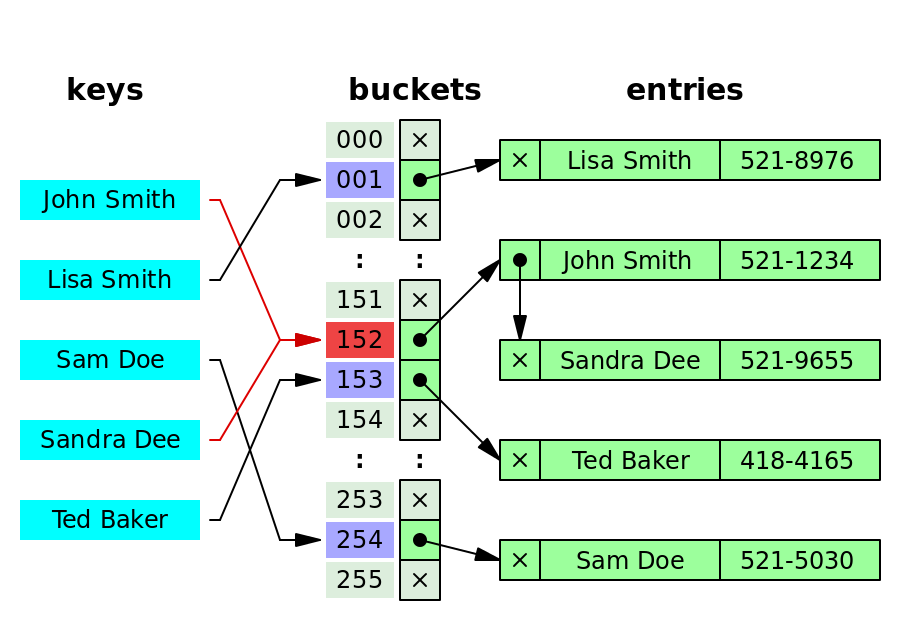
\includegraphics[width=\textwidth]{figures/Wikipedia_hash_table.png}
\vskip1em
\end{column}
\end{columns}

\vspace*{-0.1em}
are the attributes of the primary key, and the \textbf{\alert{values}} are the entire tuples themselves.

\vskip1em
\end{frame}

%
% -------------------------------------------------------------------------------------------------------
%

\begin{frame}

Hash tables are suitable for implementing primary keys and foreign keys efficiently.
\begin{itemize}[-]
\item They provide \emph{Expected} $O(1)$ cost for finding if a key is already in the table, which allows the DBMS to check violations to key constraints.
\end{itemize}

Hash tables are also suitable for implementing joins on primary/foreign key pairs.

\vskip1em

Hashing is also used in a DBMS to implement a set data structure, needed for duplicate elimination.

\end{frame}


%
% -------------------------------------------------------------------------------------------------------
%
\begin{frame}{Static Hashing}

\textbf{Goal}: store and retrieve tuples with \emph{expected} $O(1)$ I/O operations.

Design parameters:
\begin{itemize}[-,noitemsep,topsep=-0.5em]
\item $B$: number of \alert{\emph{buckets}}.
\item \alert{$h()$}: hash function that maps tuples into a number $0 \leq i < B$.
\end{itemize}

 \vskip1em

\begin{columns}[onlytextwidth]
\begin{column}{0.5\textwidth}
Example: $B=4$ buckets.

\vskip1em
- $h(t_1)=2$\\
- $h(t_2)=1$\\
- $h(t_3)=0$\\
- $h(t_4)=1$
\end{column}
\begin{column}{0.5\textwidth}
\setcounter{tIdCnt}{0}
\vskip1em
\scalebox{0.75}{
\begin{tikzpicture}
\staticHashBlock{b0}{0}{0};\node [left= 0.5em of b0] {0};
\staticHashBlock{b1}{0}{-1.5};\node [left= 0.5em of b1] {1};
\staticHashBlock{b2}{0}{-3};\node [left= 0.5em of b2] {2};
\staticHashBlock{b3}{0}{-4.5};\node [left= 0.5em of b3] {3};
\staticHashBlockEntry{b2}{0};
\staticHashBlockEntry{b1}{0};
\staticHashBlockEntry{b0}{0};
\staticHashBlockEntry{b1}{1};
\end{tikzpicture}}
\end{column}
\end{columns}
\end{frame}

%
% -------------------------------------------------------------------------------------------------------
%
\begin{frame}{Good Hash Functions\footnote{\url{https://en.wikipedia.org/wiki/Hash_function}}?}

A \alert{perfect} hash function has the following properties:
\begin{enumerate}[label=(\arabic*)]
\item it is \textbf{fast} to compute

\item it avoids \emph{collisions}: if $t_1 \neq t_2$ then $h(t_1)\neq h(t_2)$

\item it avoids \emph{clustering}: hash values are ``nicely'' spread in $[0, B)$
\end{enumerate}

\vskip1em

A good (and usable) hash function \emph{approximates} these properties.

Typical hash function \framebox{$h(t) = f(t)\mod B$}, where $f(t)$ computes a number out of the tuple (e.g., sum of first 20 bytes in the key).
\end{frame}


%
% -------------------------------------------------------------------------------------------------------
%
\begin{frame}{Insertions with Static Hash Files}

Every new tuple $t_i$ is stored on block $h(t_i)$. 

\vskip1em

If block $h(t_i)$ has room for another tuple, just make the insertion.

\vskip2em

\alert{If $h(t_i)$ is full}, there are two options:
\begin{enumerate}[(1)]
\item Probe subsequent buckets \textbf{sequentially} until an empty slot is found.

\item Grow the buckets with \blue{\emph{overflow} blocks}.
\end{enumerate}

\end{frame}

%
% -------------------------------------------------------------------------------------------------------
%
\begin{frame}

\textbf{Example:} insert new tuple $t_5$ with $h(t_5)=1$

\vskip2em

\begin{columns}[onlytextwidth]
\begin{column}{0.5\textwidth}
Sequential probing:

\vskip1em
\setcounter{tIdCnt}{0}
\scalebox{0.75}{
\begin{tikzpicture}
\staticHashBlock{b0}{0}{0};\node [left= 0.5em of b0] {0};
\staticHashBlock{b1}{0}{-1.5};\node [left= 0.5em of b1] {1};
\staticHashBlock{b2}{0}{-3};\node [left= 0.5em of b2] {2};
\staticHashBlock{b3}{0}{-4.5};\node [left= 0.5em of b3] {3};
\staticHashBlockEntry{b2}{0};
\staticHashBlockEntry{b1}{0};
\staticHashBlockEntry{b0}{0};
\staticHashBlockEntry{b1}{1};
\node [dataBox,yshift = - \dimexpr 0.5pt + (1pt + 1.4em),below right=0.5pt and 0.75pt of b2.north west] {$t_5$};
\draw [->,dotted,thick,color=blue] (b1.east) to [out=315,in=45] ([yshift=-10pt]b2.east);
\end{tikzpicture}}
\end{column}
\begin{column}{0.5\textwidth}
Using overflow blocks:

\vskip1em
\setcounter{tIdCnt}{0}
\scalebox{0.75}{
\begin{tikzpicture}
\staticHashBlock{b0}{0}{0};\node [left= 0.5em of b0] {0};
\staticHashBlock{b1}{0}{-1.5};\node [left= 0.5em of b1] {1};
\staticHashBlock{b2}{0}{-3};\node [left= 0.5em of b2] {2};
\staticHashBlock{b3}{0}{-4.5};\node [left= 0.5em of b3] {3};
\staticHashBlockEntry{b2}{0};
\staticHashBlockEntry{b1}{0};
\staticHashBlockEntry{b0}{0};
\staticHashBlockEntry{b1}{1};

\staticHashBlock{overflow}{3}{-1.5};
\node [dataBox,below right=0.5pt and 0.75pt of overflow.north west] {$t_5$};
\draw [->,thick,color=red] ([yshift=10pt]b1.east) to [out=0,in=180] (overflow);
\end{tikzpicture}}
\end{column}
\end{columns}
\end{frame}

%
% -------------------------------------------------------------------------------------------------------
%
\begin{frame}

\textbf{Sequential probing complicates deletions \textbf{and} searches.}

\vskip2em

\begin{columns}[onlytextwidth]
\begin{column}{0.7\textwidth}
Assume we further insert $t_6$ with $h(t_6) = 2$.

\vskip0.5em

What to do if we wish to \alert{delete} $t_5$?

\vskip2em

\textbf{Option 1:} \emph{compact} the file
\begin{itemize}[-,noitemsep,topsep=-0.5em]
\item Scan the file until the first empty slot after $t_5$.
\item Re-hash all tuples out of place in that interval.
\end{itemize}

\vskip1em

\textbf{Option 2:} put a ``tombstone'' marker (
\includegraphics[height=1em]{figures/RIP.pdf})
\begin{itemize}[-,noitemsep,topsep=-0.5em]
\item \textbf{Ignore tombstones} when \textbf{\alert{searching}}
\item Re-use the spot if possible
\end{itemize}


\end{column}
\begin{column}{0.25\textwidth}
\setcounter{tIdCnt}{0}
\scalebox{0.75}{
\begin{tikzpicture}
\staticHashBlock{b0}{0}{0};\node [left= 0.5em of b0] {0};
\staticHashBlock{b1}{0}{-1.5};\node [left= 0.5em of b1] {1};
\staticHashBlock{b2}{0}{-3};\node [left= 0.5em of b2] {2};
\staticHashBlock{b3}{0}{-4.5};\node [left= 0.5em of b3] {3};
\staticHashBlockEntry{b2}{0};
\staticHashBlockEntry{b1}{0};
\staticHashBlockEntry{b0}{0};
\staticHashBlockEntry{b1}{1};
\node [dataBox,yshift = - \dimexpr 0.5pt + (1pt + 1.4em),below right=0.5pt and 0.75pt of b2.north west] {$t_5$};
\draw [->,dotted,thick,color=blue] (b1.east) to [out=315,in=45] ([yshift=-10pt]b2.east);

\node [dataBox,below right=1pt and 0.75pt of b3.north west] {$t_6$};
\draw [->,dotted,thick,color=magenta] (b2.east) to [out=315,in=45] ([yshift=5pt]b3.east);
\end{tikzpicture}}
\end{column}
\end{columns}
\end{frame}

%
% -------------------------------------------------------------------------------------------------------
%
\begin{frame}

\textbf{Overflow blocks complicate deletions \textbf{and} searches.}

\vskip1em

Assume we further insert $t_5, t_6$ and $t_7$ with $h(t_5) = h(t_6) = h(t_7) = 1$.

\vskip0.5em

What to do if we wish to \alert{delete} $t_5$?

\vskip2em

\begin{columns}[onlytextwidth]
\begin{column}{0.45\textwidth}

\textbf{Option 1:} \emph{compact} the file
\begin{itemize}[-,topsep=-0.5em]
\item May require moving tuples through many blocks
\end{itemize}

\vskip1em

\textbf{Option 2:} leave gaps
\begin{itemize}[-,topsep=-0.5em]
\item Reduces I/O efficiency when searching
\end{itemize}

\end{column}
\begin{column}{0.5\textwidth}
\setcounter{tIdCnt}{0}
\scalebox{0.75}{
\begin{tikzpicture}
\staticHashBlock{b0}{0}{0};\node [left= 0.5em of b0] {0};
\staticHashBlock{b1}{0}{-1.5};\node [left= 0.5em of b1] {1};
\staticHashBlock{b2}{0}{-3};\node [left= 0.5em of b2] {2};
\staticHashBlock{b3}{0}{-4.5};\node [left= 0.5em of b3] {3};
\staticHashBlockEntry{b2}{0};
\staticHashBlockEntry{b1}{0};
\staticHashBlockEntry{b0}{0};
\staticHashBlockEntry{b1}{1};

\staticHashBlock{overflow}{2.75}{-1.5};
\node [dataBox,below right=0.5pt and 0.75pt of overflow.north west] {$t_5$};
\node [dataBox,yshift = - \dimexpr 0.5pt + (1pt + 1.4em),below right=0.5pt and 0.75pt of overflow.north west] {$t_6$};
\draw [->,thick,color=red] ([yshift=10pt]b1.east) to [out=0,in=180] (overflow);

\staticHashBlock{overflow2}{5.5}{-1.5};
\node [dataBox,below right=0.5pt and 0.75pt of overflow2.north west] {$t_7$};
\draw [->,thick,color=red] ([yshift=10pt]overflow.east) to [out=0,in=180] (overflow2);
\end{tikzpicture}}
\end{column}
\end{columns}

\end{frame}

%
% -------------------------------------------------------------------------------------------------------
%
\begin{frame}{I/O cost of Static Hashing}

\textbf{Best case scenario} (one block per bucket and no collisions): the cost of all operations (insertion, search, and deletion) is 1 I/O operation.

\vskip1em

The analysis of the \textbf{average} case cost (with some collisions) gives the same cost for both probing or using overflow chains: $O(\log N)$ for all operations, where $N$ is the number of records in the file.

The same is true for hash file in memory!


\end{frame}

%
% -------------------------------------------------------------------------------------------------------
%
\begin{frame}{Static hashing does not scale}

Static hashing works reasonably well as long as a fraction of blocks that are used remains relatively low (usually, below 75\%).

If the file gets ``too full'' we need to:
\begin{enumerate}[(1),topsep=-0.5em]
\item Add more buckets (increasing $B$)
\item \alert{Re-hash every tuple!} (because $B$ increased!)
\end{enumerate}

\vskip1em

\begin{BOX}{Know your programming language}
In-memory implementations of hash sets and dictionaries/maps in Python and Java use static hashing that grow by \textbf{doubling} in size whenever they are ``too full''.
\end{BOX}


\end{frame}

%
% -------------------------------------------------------------------------------------------------------
%
\begin{frame}{Dynamic Hashing}

Static hashing is bad because growing the hash file is very expensive... requiring to re-hash everything again after certain updates, which can take a very long time.

\vskip2em

\textbf{Dynamic hashing} schemes aim to \alert{grow the hash file incrementally}.

\alert{\textbf{Extensible Hashing}} keeps a dynamic in-memory directory with pointers to disk blocks. (See 11.7 in Silberschatz et al. or 11.3.5 in Garcia-Molina et al.)

\alert{\textbf{Linear Hashing}} grows the hash file one block at a time.

\end{frame}

%
%%!TEX root = ./lec04_access_methods.tex

%
% -------------------------------------------------------------------------------------------------------
%
\begin{frame}{Extensible hashing}

Two ingredients:

\begin{enumerate}[label=(\arabic*)]
\item keep a \textbf{directory} mapping \emph{logical buckets} into physical buckets (i.e., disk blocks)

\item the hash function computes a sequence of $k$ bits (e.g., $k=64$); but only the \alert{first $i$} bits are used to number the logical buckets
\end{enumerate}

\textbf{Example:} $k=4$ and $i=1$

\begin{center}
\setcounter{tIdCnt}{0}
\scalebox{0.75}{
\begin{tikzpicture}
\directory{d}{0}{-1}{1};
\extensibleHashBlock{b0}{2}{0}{1}
\extensibleHashBlock{b1}{2}{-2}{1}
\hashLink{d}{0}{b0}
\hashLink{d}{1}{b1}
\dynamicHashBlockEntry{b0}{0}{0110}{$t_1$}
\dynamicHashBlockEntry{b1}{0}{1011}{$t_2$}
\dynamicHashBlockEntry{b0}{1}{0011}{$t_3$}
\end{tikzpicture}}
\end{center}
\end{frame}


%
% -------------------------------------------------------------------------------------------------------
%
\begin{frame}{Insertion with Extensible Hashing}

Like before, every new tuple $t_i$ goes into bucket $h(t_i)$.

\vskip1em

\textbf{Example:} insert $t_4$ with $h(t_4) = 1001$. 

\vskip1em

\begin{center}
\setcounter{tIdCnt}{0}
\scalebox{0.75}{
\begin{tikzpicture}
\extensibleHashBlock{b0}{2}{0}{1}
\extensibleHashBlock{b1}{2}{-2}{1}
\dynamicHashBlockEntry{b0}{0}{0110}{$t_1$}
\dynamicHashBlockEntry{b1}{0}{1011}{$t_2$}
\dynamicHashBlockEntry{b0}{1}{0011}{$t_3$}


\only<1-2|handout:1>{
	\directory{d}{0}{-1}{1};
	\hashLink{d}{0}{b0}
	\hashLink{d}{1}{b1}
}

\only<2|handout:1>{
	\dynamicHashBlockEntry{b1}{1}{1001}{$t_4$};

	\node (0) at (2.25,-2.8) [thick,color=red,draw,rectangle,minimum height = 1.25em,minimum width = 1.25em] {};
	\node (1) at (-0.45,-1.8) [thick,color=red,draw,rectangle,minimum height = 1.25em,minimum width = 1.25em] {};
	\draw [->,thick, color=red] (0) -- (1);
}
\end{tikzpicture}}
\end{center}
\end{frame}


%
% -------------------------------------------------------------------------------------------------------
%
\begin{frame}

Inserting a tuple into a bucket that is already full forces the \textbf{directory} to grow, by \framebox{increasing \alert{$i$}}.


\vskip1em

\textbf{Example:} insert $t_5$ with $h(t_5) = 0100$. 

\vskip1em

\begin{center}
\setcounter{tIdCnt}{0}
\scalebox{0.75}{
\begin{tikzpicture}
	\extensibleHashBlock{b1}{2}{-4}{1}
	\dynamicHashBlockEntry{b1}{0}{1011}{$t_2$}
	\dynamicHashBlockEntry{b1}{1}{1001}{$t_4$}

\only<1|handout:0>{
	\directory{d}{0}{-1}{1};
	\extensibleHashBlock{b0}{2}{0}{1}	
	\hashLink{d}{0}{b0}
	\hashLink{d}{1}{b1}
	\dynamicHashBlockEntry{b0}{0}{0110}{$t_1$}
	\dynamicHashBlockEntry{b0}{1}{0011}{$t_3$}
}

\only<2-3|handout:1>{
	\directory{d}{0}{-2}{2};
	\extensibleHashBlock{b00}{2}{0}{2}
	\extensibleHashBlock{b01}{2}{-2}{2}

	\hashLink{d}{0}{b00}
	\hashLink{d}{1}{b01}
	\hashLink{d}{2}{b1}
	\hashLink{d}{3}{b1}

	\dynamicHashBlockEntry{b01}{0}{0110}{$t_1$}
	\dynamicHashBlockEntry{b01}{1}{0100}{$t_5$}
	\dynamicHashBlockEntry{b00}{0}{0011}{$t_3$}
}

\only<3|handout:0>{
	\coordinate [left= 1cm of b00] (0) ;
	\draw [->,very thick,color=blue] ([yshift=1em]0) -- ([yshift=5pt]b00.north west);

	\coordinate [left= 1cm of b01] (1) ;
	\draw [->,very thick,color=blue] ([yshift=1em]1) -- ([yshift=5pt]b01.north west);

	\draw [color=red,decorate,decoration={brace,amplitude=5pt,raise=8pt},yshift=0pt]
		(-0.5,-4.2) -- (-0.5,-3) node [midway,xshift=-2.5cm] {
	\begin{minipage}{3.5cm}\baselineskip=0.75\baselineskip \centering
		two logical buckets sharing the same physical bucket
	\end{minipage}
		};
}
\end{tikzpicture}}
\end{center}
\end{frame}


%
% -------------------------------------------------------------------------------------------------------
%
\begin{frame}

\textbf{Example:} insert $t_6$ with $h(t_6) = 0100$. 

\vskip1em

\begin{center}
\setcounter{tIdCnt}{0}
\scalebox{0.75}{
\begin{tikzpicture}
	\extensibleHashBlock{b00}{2}{0}{2}
	\extensibleHashBlock{b1}{2}{-6}{1}
	\dynamicHashBlockEntry{b1}{0}{1011}{$t_2$}
	\dynamicHashBlockEntry{b1}{1}{1001}{$t_4$}
	\dynamicHashBlockEntry{b00}{0}{0011}{$t_3$}

\only<1|handout:0>{
	\directory{d}{0}{-2}{2};

	\extensibleHashBlock{b01}{2}{-2}{2}

	\hashLink{d}{0}{b00}
	\hashLink{d}{1}{b01}
	\hashLink{d}{2}{b1}
	\hashLink{d}{3}{b1}

	\dynamicHashBlockEntry{b01}{0}{0110}{$t_1$}
	\dynamicHashBlockEntry{b01}{1}{0100}{$t_5$}
}

\only<2|handout:1>{
	\directory{d}{0}{-2.5}{3};
	\extensibleHashBlock{b010}{2}{-2}{3}
	\extensibleHashBlock{b011}{2}{-4}{3}

	\hashLink{d}{0}{b00}
	\hashLink{d}{1}{b00}
	\hashLink{d}{2}{b010}
	\hashLink{d}{3}{b011}
	\hashLink{d}{4}{b1}
	\hashLink{d}{5}{b1}
	\hashLink{d}{6}{b1}
	\hashLink{d}{7}{b1}

	\dynamicHashBlockEntry{b011}{0}{0110}{$t_1$}
	\dynamicHashBlockEntry{b010}{0}{0100}{$t_5$}
	\dynamicHashBlockEntry{b010}{1}{0100}{$t_6$}
}
\end{tikzpicture}}
\end{center}
\end{frame}

\newsavebox{\dynamicHashingExample}
\savebox{\dynamicHashingExample}{
\begin{tikzpicture}
	\directory{d}{0}{-2.5}{3};
	\extensibleHashBlock{b010}{2}{-2}{3}
	\extensibleHashBlock{b011}{2}{-4}{3}
	\extensibleHashBlock{b00}{2}{0}{2}
	\extensibleHashBlock{b1}{2}{-6}{1}

	\hashLink{d}{0}{b00}
	\hashLink{d}{1}{b00}
	\hashLink{d}{2}{b010}
	\hashLink{d}{3}{b011}
	\hashLink{d}{4}{b1}
	\hashLink{d}{5}{b1}
	\hashLink{d}{6}{b1}
	\hashLink{d}{7}{b1}

	\dynamicHashBlockEntry{b1}{0}{1011}{$t_2$}
	\dynamicHashBlockEntry{b1}{1}{1001}{$t_4$}
	\dynamicHashBlockEntry{b00}{0}{0011}{$t_3$}
	\dynamicHashBlockEntry{b011}{0}{0110}{$t_1$}
	\dynamicHashBlockEntry{b010}{0}{0100}{$t_5$}
	\dynamicHashBlockEntry{b010}{1}{0100}{$t_6$}
\end{tikzpicture}}

%
% -------------------------------------------------------------------------------------------------------
%
\begin{frame}{Deletions with Extensible Hashing}

Deletions are only an issue if they cause a \textbf{physical} bucket to become empty.

\textbf{Example:} delete tuple $t_1$ with $h(t_1)=0110$.

\vskip1em

\begin{columns}[onlytextwidth]
\begin{column}{0.6\textwidth}
\textbf{Option 1:} \alert{merge logical buckets} (010 and 011 in this case); \alert{shrink the directory} (decrease $i$) if needed\footnotemark.

\vskip1em

\textbf{Option 2:} put a ``tombstone'' mark (
\includegraphics[height=1em]{images/RIP.pdf}) in place of $t_1$. Re-build table when database goes offline for maintenance.
\end{column}
\begin{column}{0.3\textwidth}
\scalebox{0.5}{\usebox\dynamicHashingExample}
\end{column}
\end{columns}
\vskip1em

\footnotetext{Not all deletions lead to shrinking the directory. For example, there would be no shrinking if logical buckets 000 and 001 were on separate physical buckets.}
\end{frame}

%
% -------------------------------------------------------------------------------------------------------
%
\begin{frame}{Too Many Collisions can Break Extensible Hashing}

\textbf{Example:} how to handle the insertion of $t_7$ with $h(t_7)=0100$? 

When more tuples hash to the same bucket than a physical bucket can fit, further growing the directory doesn't help.

\vskip1em

\begin{columns}[onlytextwidth]
\begin{column}{0.6\textwidth}
\textbf{Option 1:} start an \alert{overflow chain} on the block with $t_5$ and $t_6$.

\vskip1em

\textbf{Option 2:} add a level of indirection with ``bucket files''\footnotemark as was done for secondary indexes (slide~\ref{bucket_files_secondary_indexes}). This increases I/O cost.
\end{column}
\begin{column}{0.3\textwidth}
\scalebox{0.5}{\usebox\dynamicHashingExample}
\end{column}
\end{columns}

\footnotetext{Not to be confused with the ``hashing buckets''.}

\end{frame}

%
% -------------------------------------------------------------------------------------------------------
%
\begin{frame}{Extensible Hashing: Summary}

\textbf{Pros:}\\
 - without duplicates, physical buckets are always 1 disk block\\
 - all operations require $O(1)$ I/O (if directory can fit in memory)\\
 - ``file'' on disk grows one block at a time

\textbf{Cons:}\\
 - need to keep directory in memory (or do more I/O)\\
 - directory grows exponentially
 
\vskip1em

\textbf{Worst problem of extensible hashing}: a ``bad'' hash function can cause the directory to grow very big (very fast). Suppose $k=32$ and the number of tuples per bucket is 2 (as in the running example). If there are 3 tuples whose hash values disagree on their $20^{\mathit{th}}$ bit, the directory will grow to $2^{20}$ entries to hold them.
\end{frame}

%
% -------------------------------------------------------------------------------------------------------
% 
%

%
% -------------------------------------------------------------------------------------------------------
%
\begin{frame}{Linear Hashing}

Four ingredients:

\begin{enumerate}[label=(\arabic*)]

\item Distinguish between \emph{virtual} and \emph{materialized} buckets.

\item Use the \alert{last $i$} bits of the hash value as the bucket number.\\[0.5em] If a tuple hashes to a virtual bucket, use the last $i-1$ bits instead (which is guaranteed to map to a materialized bucket).

\item Buckets can span multiple disk blocks (using overflow chains).

\item Add more materialized buckets once the load factor goes over a threshold.
\end{enumerate}
\end{frame}

%
% -------------------------------------------------------------------------------------------------------
%
\begin{frame}

\textbf{Example:} $k=4$ and $i=1$ (meaning, two logical blocks).

\begin{center}

\vskip2em

\scalebox{0.75}{
	\begin{tikzpicture}
	\linearHashVariables{0}{0}{1}{2}{3}
	\linearHashBlock{b0}{3}{0}{0}
	\linearHashBlock{b1}{3}{-1.1}{1}
	\dynamicHashBlockEntry{b0}{0}{0000}{$t_1$}
	\dynamicHashBlockEntry{b0}{1}{1010}{$t_3$}
	\dynamicHashBlockEntry{b1}{0}{1011}{$t_2$}

	\node (0) at (-3,-0.75) [color=red] {
		\begin{minipage}{4cm}\baselineskip=0.75\baselineskip \centering
		number of physical buckets
	\end{minipage}
	};
	\draw[->,color=red,thick] (0) -- (0,-1.15);
	\node (1) at (-2.25,-2.25) [color=blue] {
		\begin{minipage}{2.5cm}\baselineskip=0.75\baselineskip \centering
		number of records in file
	\end{minipage}
	};
	\draw[->,color=blue,thick] (1) -- (0,-2);
	\end{tikzpicture}
}

\vskip3em 

Invariants: \framebox{$i=\ceil{\log_2 n}$} and \framebox{$r/n \leq C \cdot|\text{block}|$}
\end{center}

\vskip1em

$C$ is the \textbf{load factor} above which the file must grow. 

In the example, $|\text{block}|=2$ and the file must grow if $r/n > 1.7$ for a maximum load factor of $C=85\%$.
\end{frame}

%
% -------------------------------------------------------------------------------------------------------
%
\begin{frame}{Finding the bucket of a tuple}
\label{physical_block_in_linear_hashing}

The \alert{\emph{logical} bucket} of tuple $t_i$ is the integer \alert{$m$} corresponding to the \alert{lowest $i$ bits in $h(t_i)$}. 

(1) \alert{$m < n$}: the logical bucket is materialized.\\
 In this case, the \textbf{bucket} of $t_i$ is $m$ itself.

(2) \alert{$m \geq n$}: the logical bucket is virual (i.e., it is not on disk yet).\\
 In this case, the \textbf{bucket} of $t_i$ is the one corresponding to the lowest $i-1$ bits in $h(t_i)$).

\vskip1em

\begin{BOX}{Invariant}
Every tuple has a \textbf{bucket} where it gets stored, even if we do not use all $i$ bits of the hash value.
\end{BOX}
\end{frame}

%
% -------------------------------------------------------------------------------------------------------
%
\begin{frame}{Insertions With Linear Hashing}

\textbf{Algorithm} for inserting tuple $t_i$ into a Linear Hash file

\begin{enumerate}[label=(\arabic*)]
\item determine the \textbf{bucket} of $t_i$ (slide~\ref{physical_block_in_linear_hashing})
\item if the bucket has room, add $t_i$; otherwise, \blue{grow the bucket using an overflow block} and add $t_i$
\item \alert{increase $r$}
\item \alert{if $r/n > C\cdot|\text{block}|$}, add one more bucket to the file and increase $n$ \\[0.5em]\alert{if $\ceil{\log_2 n}>i$}, increase $i$ and \alert{re-hash} the tuples in physical block $n-2^i$
\end{enumerate}
\end{frame}

%
% -------------------------------------------------------------------------------------------------------
%
\begin{frame}

\textbf{Example:} inserting $t_4$ with $h(t_4)=0101$

\vskip2em

\begin{center}
\scalebox{0.75}{
	\begin{tikzpicture}

\only<1|handout:1>{
	\linearHashVariables{0}{0}{1}{2}{3}
}
	\linearHashBlock{b0}{3}{0}{0}
	\linearHashBlock{b1}{3}{-1.1}{1}
	\dynamicHashBlockEntry{b0}{0}{0000}{$t_1$}
	\dynamicHashBlockEntry{b0}{1}{1010}{$t_3$}
	\dynamicHashBlockEntry{b1}{0}{1011}{$t_2$}

\only<2|handout:2>{
	\linearHashVariables{0}{0}{1}{2}{4}
	\dynamicHashBlockEntry{b1}{1}{0101}{$t_4$}

	\node (0) at (-2.5,-1.5) [color=red] {$r/n=2>1.7$};
}
	\end{tikzpicture}
}
\end{center}

\vskip2em

\only<2|handout:2>{
	With the insertion, the load factor is too high and the file needs to grow (next slide).
}
\end{frame}

%
% -------------------------------------------------------------------------------------------------------
%
\begin{frame}{Growing the file; $i$ Increases}
\label{linear_hashing_increase_i}

Adding a bucket makes \alert{$n=3$}; since $\ceil{\log_2 3} > 1$, $i$ is increased, \textbf{doubling} the space of \emph{logical bucket} addresses:
\begin{itemize}[-,noitemsep,topsep=-0.5em]
\item The ``lower half'' of the space has the old buckets
\item The new bucket becomes the \textbf{first} in the ``upper half'': \textcolor{red}{1}$0_{i-1}\cdots 0_0$.
\item We must check for tuples ``out of place'' in \textcolor{red}{0}$0_{i-1}\cdots 0_0$
\end{itemize}

\begin{center}
\vskip1em

\scalebox{0.75}{
	\begin{tikzpicture}

	\linearHashVariables{0}{0}{2}{3}{4}
	\linearHashBlock{b00}{3}{0}{\textcolor{red}{0}0}
	\linearHashBlock{b01}{3}{-1.1}{\textcolor{red}{0}1}
	\linearHashBlock{b10}{3}{-2.2}{\textcolor{red}{1}0}
	\missingLinearHashBlock{b11}{3}{-3.35}{\textcolor{fern}{11}}

	\dynamicHashBlockEntry{b00}{0}{0000}{$t_1$}
	\dynamicHashBlockEntry{b01}{1}{0101}{$t_4$}
	\dynamicHashBlockEntry{b01}{0}{1011}{$t_2$}

\only<1|handout:1>{
	\dynamicHashBlockEntry{b00}{1}{1010}{$t_3$}

	\draw[thick,->,dotted,blue] (b10.east) to [out=15,in=345] (b00.east);

	\node [right=2em of b01,blue] {
		\begin{minipage}{3cm}\baselineskip=0.75\baselineskip \centering \small
		must check for tuples \textbf{ending in 10}
	\end{minipage}
	};
	\node [right of=b11,xshift=-3em,color=fern] {\small not yet added};
}

\only<2|handout:2>{
	\dynamicHashBlockEntry{b10}{0}{1010}{$t_3$}	
	\draw[thick,->,dotted,blue] ([yshift=-5pt]b00.east) to [in=15,out=345] ([yshift=5pt]b10.east);
}
	\end{tikzpicture}}
\end{center}
\end{frame}

%
% -------------------------------------------------------------------------------------------------------
%
\begin{frame}

\begin{block}{Re-hashing tuples out of place}
Whenever we add a new materialized bucket (even when $i$ remains unchanged), we must check for tuples out of place and move them accordingly.
\end{block}

\vskip1em

Let the new materialized bucket be at binary address $\alert{1}\blue{b_{i-1}\cdots b_{0}}$. 

Note that, \underline{prior to adding this block}, any tuple with that exact hash value would have been inserted using less than $i$ bits!

Those tuples would be in the bucket with address $\alert{0}\blue{b_{i-1}\cdots b_{0}}$.

\end{frame}



%
% -------------------------------------------------------------------------------------------------------
%
\begin{frame}
When adding an \alert{overflow} block; $n$ and $i$ stay the same\\

\vskip1em

\textbf{Example:} adding tuple $t_5$ with $h(t_5)=1111$

\begin{center}

\vskip1em

\scalebox{0.75}{
	\begin{tikzpicture}
	\linearHashBlock{b00}{3}{0}{00}
	\linearHashBlock{b01}{3}{-1.1}{01}
	\linearHashBlock{b10}{3}{-2.2}{10}
	\missingLinearHashBlock{b11}{3}{-3.35}{\textcolor{fern}{11}}

	\dynamicHashBlockEntry{b00}{0}{0000}{$t_1$}
	\dynamicHashBlockEntry{b01}{1}{0101}{$t_4$}
	\dynamicHashBlockEntry{b01}{0}{1011}{$t_2$}
	\dynamicHashBlockEntry{b10}{0}{1010}{$t_3$}	

\only<1|handout:1>{
	\linearHashVariables{0}{0}{2}{3}{4}
	\node [right of=b11,xshift=-3em,color=fern] {\small not yet added};
}

\only<2|handout:2>{
	\linearHashVariables{0}{0}{2}{3}{5}
	\linearHashBlock{overflow}{7}{-1.1}{}
	\dynamicHashBlockEntry{overflow}{0}{1111}{$t_5$}

	\draw[->,>=stealth',thick,red] ([yshift=8pt]b01.east) to [out=0,in=180] (overflow);
}
	\end{tikzpicture}}

\vskip1em

\framebox{$n$ \textbf{\alert{does not increase}} when adding an overflow block}

\end{center}
\end{frame}

%
% -------------------------------------------------------------------------------------------------------
%
\begin{frame}

\textbf{Another example} of inserting into empty slots: add tuple $t_6$ with $h(t_6)=0111$

\vskip1em

\begin{center}

\scalebox{0.75}{
	\begin{tikzpicture}

	\linearHashVariables{0}{0}{2}{3}{6}
	\linearHashBlock{b00}{3}{0}{00}
	\linearHashBlock{b01}{3}{-1.1}{01}
	\linearHashBlock{b10}{3}{-2.2}{10}
	\missingLinearHashBlock{b11}{3}{-3.35}{\textcolor{fern}{11}}

	\dynamicHashBlockEntry{b00}{0}{0000}{$t_1$}
	\dynamicHashBlockEntry{b01}{1}{0101}{$t_4$}
	\dynamicHashBlockEntry{b01}{0}{1011}{$t_2$}
	\dynamicHashBlockEntry{b10}{0}{1010}{$t_3$}	

	\linearHashBlock{overflow}{7}{-1.1}{}
	\draw[->,>=stealth',thick,red] ([yshift=8pt]b01.east) to [out=0,in=180] (overflow);
	\dynamicHashBlockEntry{overflow}{0}{1111}{$t_5$}
	\dynamicHashBlockEntry{overflow}{1}{0111}{$t_6$}

	\node (0) at (-2.5,-1.5) [color=red] {$r/n=2>1.7$};

	\end{tikzpicture}}
\end{center}
\vskip2em
With the insertion, the load factor is too high and the file needs to grow (next slide).
\end{frame}

%
% -------------------------------------------------------------------------------------------------------
%
\begin{frame}{Growing the file; $i$ Stays the Same}

\vskip2em

\begin{center}

\scalebox{0.75}{
	\begin{tikzpicture}

\only<1|handout:1>{
	\linearHashVariables{0}{0}{2}{3}{6}
	\dynamicHashBlockEntry{b01}{0}{1011}{$t_2$}
	\dynamicHashBlockEntry{b01}{1}{0101}{$t_4$}
	\linearHashBlock{overflow}{7}{-1.1}{}
	\draw[->,>=stealth',thick,red] ([yshift=8pt]b01.east) to [out=0,in=180] (overflow);
	\dynamicHashBlockEntry{overflow}{0}{1111}{$t_5$}
	\dynamicHashBlockEntry{overflow}{1}{0111}{$t_6$}

	\draw[thick,->,dotted,blue] (b11.east) to [out=15,in=345] (b01.east);
	\node [right=2em of b11,blue] {
		\begin{minipage}{3cm}\baselineskip=0.75\baselineskip \centering \small
		must check for tuples \textbf{ending in 11} (including the overflow block!)
	\end{minipage}
	};

}
	\linearHashBlock{b00}{3}{0}{00}
	\linearHashBlock{b01}{3}{-1.1}{01}
	\linearHashBlock{b10}{3}{-2.2}{10}
	\linearHashBlock{b11}{3}{-3.35}{\textcolor{red}{11}}

	\dynamicHashBlockEntry{b00}{0}{0000}{$t_1$}
	\dynamicHashBlockEntry{b10}{0}{1010}{$t_3$}	

\only<2|handout:2>{
	\linearHashVariables{0}{0}{2}{4}{6}

	\dynamicHashBlockEntry{b01}{0}{0101}{$t_4$}
	\dynamicHashBlockEntry{b11}{0}{1011}{$t_2$}
	\dynamicHashBlockEntry{b11}{1}{1111}{$t_5$}
	
	\linearHashBlock{overflow}{7}{-3.35}{}
	\draw[->,>=stealth',thick,red] ([yshift=8pt]b11.east) to [out=0,in=180] (overflow);

	\dynamicHashBlockEntry{overflow}{0}{0111}{$t_6$}
}
	\end{tikzpicture}}
\end{center}

\vskip2em

\only<2|handout:2>{
With one more insertion we'd have $r=7$ and $r/n>1.7$, forcing the file to grow again ($n$ becomes 5 and $i=\ceil{\log_2 5}=3$, doubling the number of bucket addresses as in Case 1 as in slide~\ref{linear_hashing_increase_i}).
}

\end{frame}

%
% -------------------------------------------------------------------------------------------------------
%
\begin{frame}{Linear Hashing: Summary}

\textbf{Inserting duplicates?} No special treatment... just add the new tuples wherever they hash to.

\textbf{Searching?} Follow steps (1)--(3) of the insertion algorithm (slide~\ref{physical_block_in_linear_hashing}).

\textbf{Deletions?} Just put a ``tombstone'' mark (
\includegraphics[height=1em]{figures/RIP.pdf}) instead of reversing the insertion algorithm.

\vskip1em

\textbf{Access costs?}\\
 - searches, insertions and deletions require, \textbf{in expectation}, at most two I/O operations (1 read and 1 write, if the file grows).

\end{frame}


